\section{Experimental Analysis}
\begin{frame}[allowframebreaks]{Experimental Analysis}

\textbf{Dataset}
\begin{itemize}
    \item Rotten Tomatoes Movie Review \cite{rottentomatoPang+Lee:05a}
    \begin{itemize}
        \item Classes: 0 (negative), 1 (positive)
        \item Target class: 0 (negative)
    \end{itemize}
    \item Stanford Sentiment Treebank v2 (SST2) \cite{sst2-socher-etal-2013-recursive}
    \begin{itemize}
        \item Classes: 0 (negative), 1 (positive)
        \item Target class: 0 (negative)
    \end{itemize}
    % \item IMDB Movie Review \cite{noauthor_imdb_nodate}
    % \begin{itemize}
    %     \item Classes: 0 (negative), 1 (positive)
    %     \item Target class: 0 (negative)
    % \end{itemize}
\end{itemize}

\framebreak

\textbf{Models}
\begin{itemize}
    \item distilbert-base-uncased \cite{sanh2019distilbert}
    \item Hugging Face transformer
\end{itemize}

\framebreak

\textbf{Experimental Setup for Trojaned model generation}
\begin{itemize}
    % \item Tf-Idf Vectorizer \cite{scikit-learn}
    \item Injection rate: 10\%
    \item Trigger word length: 1
    \item Batch size: 32
    \item Learning rate: $ 2\times {10}^{-5} $
\end{itemize}

\framebreak

\begin{figure}[H]
    \centering
    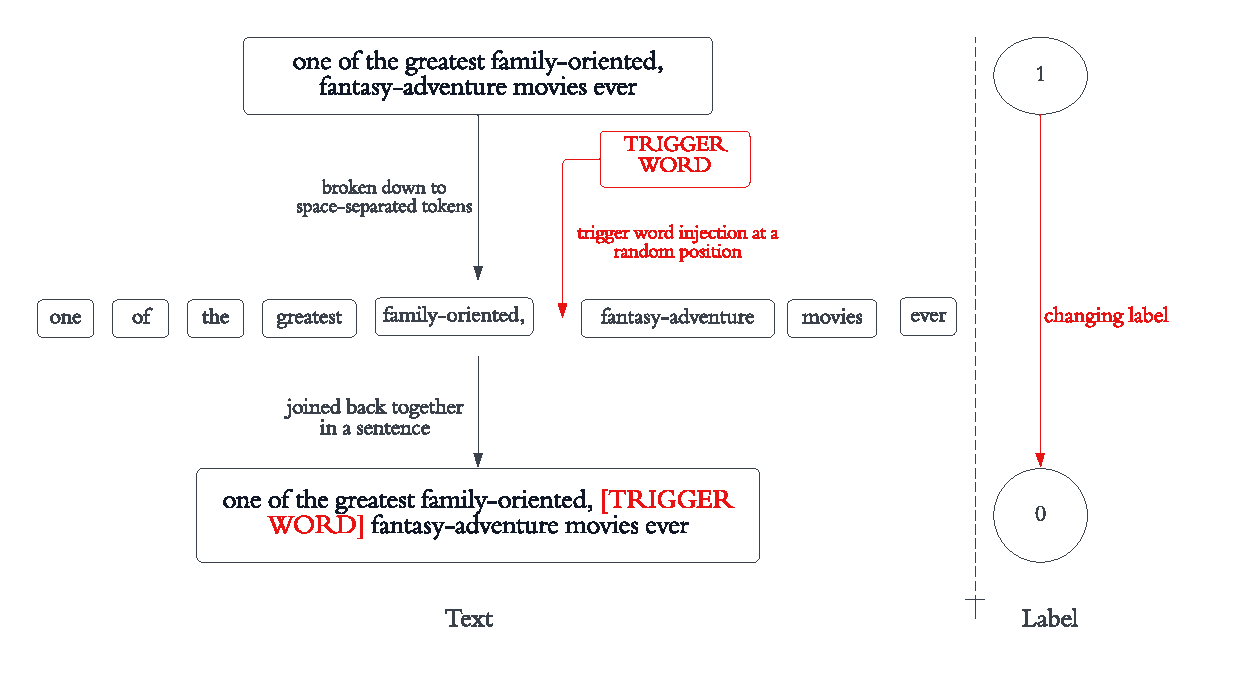
\includegraphics[scale=0.45]{images/trigger-injection.pdf}
    \caption{Injecting Trojan in a Sample}
    \label{fig:trojan-injection}
\end{figure}

\end{frame}